\documentclass[border=1pt, multi=fig]{standalone}

\usepackage{tikz}

\usetikzlibrary{positioning}

% colors
\definecolor{page}{HTML}{b8e5fe}
\definecolor{outline}{rgb}{0.6, 0.75, 0.9}

\makeatletter %@@@@@@@@@

\@ifundefined{tsp}{\pagecolor{page}}{}

% hat tip Ulrich Schwarz
% https://tex.stackexchange.com/a/5354/6934
\tikzset{nopreaction/.code=\let\tikz@preactions\pgfutil@empty}

% hat tip Andrew Stacey
% https://tex.stackexchange.com/a/47009/6934
\pgfkeys{%
  /tikz/on layer/.code={
    \pgfonlayer{#1}\begingroup
    \aftergroup\endpgfonlayer
    \aftergroup\endgroup
  },
  /tikz/node on layer/.code={
    \pgfonlayer{#1}\begingroup
    \expandafter\def\expandafter\tikz@node@finish\expandafter{\expandafter\endgroup\expandafter\endpgfonlayer\tikz@node@finish}%
  },
}

\makeatother %@@@@@@@@@

\pgfdeclarelayer{back}
\pgfsetlayers{back, main}

\tikzset{
  vwhite/.style={circle, fill=white},
  vblack/.style={circle, fill=black}
}

\newcommand{\hsep}{1.5}

% --- prototype dessin ---
\newcommand{\protovertices}{
\node[vwhite, text=black, minimum width=4mm] (w0) at (2*\hsep, -4) {};
\node[vblack, text=white, minimum width=4mm] (w1) at (3*\hsep, -4) {};
}

\newcommand{\protomidpoints}{
\coordinate (w01) at (2.5*\hsep, -4);
}

\newcommand{\protowhiteedges}{
\draw (w0.center) -- (w01);
}

\newcommand{\protoblackedges}{
\draw (w01) -- (w1.center);
}

% --- example dessin ---

\newcommand{\exvertices}{
\node[vwhite, minimum width=6mm] (v2) at (2*\hsep, 0) {};
\node[vwhite, minimum width=4mm] (v3) at (3*\hsep, 0) {};
\node[vwhite, minimum width=4mm] (v5) at (5*\hsep, 0) {};
\node[vblack, minimum width=4.5mm] (v0) at (0, 0) {};
\node[vblack, minimum width=4mm] (v1) at (1*\hsep, 0) {};
\node[vblack, minimum width=5mm] (v4) at (4*\hsep, 0) {};
}

\newcommand{\exmidpoints}{
\coordinate (v21) at (1.5*\hsep, 0);
\coordinate (v34) at (3.5*\hsep, 0);
\coordinate (v54) at (4.5*\hsep, 0);
\coordinate (v20a) at (0.85*\hsep, 1.4);
\coordinate (v20b) at (0.85*\hsep, -1.4);
\coordinate (v24a) at (3.3*\hsep, 0.9);
\coordinate (v24b) at (3.3*\hsep, -0.9);
}

\newcommand{\exwhiteedges}{
\draw (v2.center) -- (v21);
\draw (v3.center) -- (v34);
\draw (v5.center) -- (v54);
\draw (v2.center) to[out=36+72, in=0] (v20a);
\draw (v2.center) to[out=-36-72, in=0] (v20b);
\draw (v2.center) to[out=36, in=180] (v24a);
\draw (v2.center) to[out=-36, in=180] (v24b);
}

\newcommand{\exblackedges}{
\draw (v21) -- (v1.center);
\draw (v34) -- (v4.center);
\draw (v54) -- (v4.center);
\draw (v20a) to[out=180, in=90] (v0.center);
\draw (v20b) to[out=180, in=-90] (v0.center);
\draw (v24a) to[out=0, in=90] (v4.center);
\draw (v24b) to[out=0, in=-90] (v4.center);
}

\begin{document}

% dessin
\begin{fig}

\begin{tikzpicture}
% vertices
\begin{scope}[every node/.style={preaction={draw, on layer=back, line width=1mm, outline, nopreaction}}]
\exvertices
\end{scope}

% edge midpoints
\exmidpoints

% edges
\begin{scope}[line width=2mm, every path/.style={preaction={draw, on layer=back, line width=3mm, outline, nopreaction}}]
\begin{scope}[white]
\exwhiteedges
\end{scope}
\begin{scope}[black]
\exblackedges
\end{scope}
\end{scope}
\end{tikzpicture}
\end{fig}

% dessin
\begin{fig}
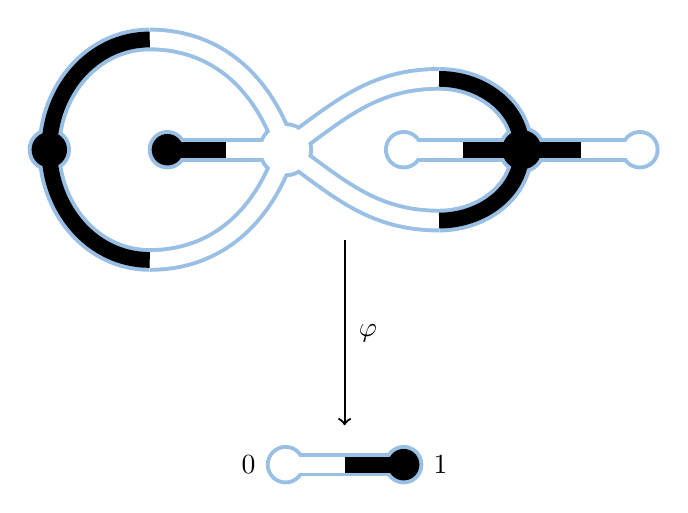
\begin{tikzpicture}
% vertices
\begin{scope}[every node/.style={preaction={draw, on layer=back, line width=1mm, outline, nopreaction}}]
\exvertices
\protovertices
\end{scope}

% edge midpoints
\exmidpoints
\protomidpoints

% edges
\begin{scope}[line width=2mm, every path/.style={preaction={draw, on layer=back, line width=3mm, outline, nopreaction}}]
\begin{scope}[white]
\exwhiteedges
\protowhiteedges
\end{scope}
\begin{scope}[black]
\exblackedges
\protoblackedges
\end{scope}
\end{scope}

% map
\draw[black,<-,thick] (w01) ++(0, 0.5) to node [right=0.5mm] {$\varphi$} ++(0, 2.35);

% labels
\node [left=0.5mm of w0] {$0$};
\node [right=0.5mm of w1] {$1$};
\end{tikzpicture}
\end{fig}

\end{document}